%%%%%%%%%%%%%%%%%%%%%%%%%%%%%%%%%%%%%%%%%
% Journal Article
% LaTeX Template
% Version 1.4 (15/5/16)
%
% This template has been downloaded from:
% http://www.LaTeXTemplates.com
%
% Original author:
% Frits Wenneker (http://www.howtotex.com) with extensive modifications by
% Vel (vel@LaTeXTemplates.com)
%
% License:
% CC BY-NC-SA 3.0 (http://creativecommons.org/licenses/by-nc-sa/3.0/)
%
%%%%%%%%%%%%%%%%%%%%%%%%%%%%%%%%%%%%%%%%%

%----------------------------------------------------------------------------------------
%	PACOTES E OUTRAS CONFIGURACOES DO DOCUMENTO
%----------------------------------------------------------------------------------------

\documentclass[
	twoside,				% frete e verso
	twocolumn,				% coluna dupla
	english,				% idioma adicional para hifenização
	brazil,					% o último idioma é o principal do documento
]{article}

% ---
% PACOTES
% ---

% ---
% Pacotes fundamentais 
% ---
\usepackage{cmap}			% Mapear caracteres especiais no PDF
\usepackage{lmodern}		% Usa a fonte Latin Modern			
\usepackage[T1]{fontenc}	% Selecao de codigos de fonte.
\usepackage[utf8]{inputenc}	% Codificacao do documento (conversão automática dos acentos)
\usepackage{indentfirst}	% Indenta o primeiro parágrafo de cada seção.
\usepackage{color}			% Controle das cores
\usepackage{graphicx}		% Inclusão de gráficos
\usepackage{lipsum}			% para geração de dummy text
\usepackage{blindtext}		% Package to generate dummy text throughout this template 
\usepackage{amsmath}

\usepackage[sc]{mathpazo}	% Use the Palatino font
\usepackage[T1]{fontenc}	% Use 8-bit encoding that has 256 glyphs
\linespread{1.05}			% Line spacing - Palatino needs more space between lines
\usepackage{microtype}		% Slightly tweak font spacing for aesthetics

\usepackage[brazil]{babel}	% Hifenizacao textual de regras tipograficas em portugues

\usepackage[hmarginratio=1:1,top=32mm,columnsep=20pt]{geometry} % Document margins
\usepackage[hang, small,labelfont=bf,up,textfont=it,up]{caption} % Custom captions under/above floats in tables or figures
\usepackage{booktabs} % Horizontal rules in tables

\usepackage{lettrine} % The lettrine is the first enlarged letter at the beginning of the text

\usepackage{enumitem} % Customized lists
\setlist[itemize]{noitemsep} % Make itemize lists more compact

\usepackage{abstract} % Allows abstract customization
\renewcommand{\abstractnamefont}{\normalfont\bfseries} % Set the "Abstract" text to bold
\renewcommand{\abstracttextfont}{\normalfont\small\itshape} % Set the abstract itself to small italic text

\usepackage{titlesec} % Allows customization of titles
\renewcommand\thesection{\Roman{section}} % Roman numerals for the sections
\renewcommand\thesubsection{\roman{subsection}} % roman numerals for subsections
\titleformat{\section}[block]{\large\scshape\centering}{\thesection.}{1em}{} % Change the look of the section titles
\titleformat{\subsection}[block]{\large}{\thesubsection.}{1em}{} % Change the look of the section titles

\usepackage{fancyhdr} % Headers and footers
\pagestyle{fancy} % All pages have headers and footers
\fancyhead{} % Blank out the default header
\fancyfoot{} % Blank out the default footer
\fancyhead[C]{Implementação de um controlador \textit{fuzzy} para um sistema de taques acoplados $\bullet$ Outubro 2016} % Custom header text
\fancyfoot[RO,LE]{\thepage} % Custom footer text

\usepackage{titling} % Customizing the title section

\usepackage{hyperref} % For hyperlinks in the PDF

%----------------------------------------------------------------------------------------
%	TITULO DA SECAO
%----------------------------------------------------------------------------------------

\setlength{\droptitle}{-4\baselineskip} % Move the title up

\pretitle{\begin{center}\Huge\bfseries} % Article title formatting
\posttitle{\end{center}} % Article title closing formatting
\title{Implementação de um Controlador Fuzzy para um sistema de taques acoplados: um estudo de caso.}
\author{
\textit{Fernando Fernandes}\thanks{\textbf{Fernando Fernandes}, Departamento de Computação e Automação, Centro de Tecnologia. \href{mailto:leandes@gmail.com}{leandes@gmail.com}} / 
\textit{Tiago Batista}\thanks{\textbf{Tiago Batista}, Departamento de Computação e Automação, Centro de Tecnologia. \href{mailto:ekyidag@gmail.com}{ekyidag@gmail.com}} / 
\textit{Rosenildo Pereira}\thanks{\textbf{Rosenildo Pereira}, Departamento de Computação e Automação, Centro de Tecnologia. \href{mailto:reidesgm@hotmail.com}{reidesgm@hotmail.com}} \\ [1ex]
\textsc{Universidade Federal do Rio Grande do Norte} \\
}
\date{\today} % Leave empty to omit a date
\renewcommand{\maketitlehookd}{%
\begin{abstract}
\noindent Este estudo aborda a configuração de um controlador PID \textit{fuzzy} utilizando os modelos de Sugeno e Mamdani para o controle de um sistema de tanques acoplados. Esta atividade foi desenvolvida utilizando o toolbox Fuzzy do Matlab R2016a Student e um modelo fornecido do Simulink. O objetivo do estudo é obter parâmetros de operação ótimos para o controlador PID dadas as condições de operação, considerando o erro entre o setpoint e o nível presente na planta, bem como a variação desse erro. Esta atividade foi proposta pelo Professor Dr. Fábio Meneghetti no escopo do componente Controle Fuzzy de Sistemas Dinâmicos do curso de Engenharia Mecatrônica da Universidade Federal do Rio Grande do Norte.

\vspace{0.4cm}
\textbf{Palavras-chave}: Lógica \textit{fuzzy}, Controle proporcional-integrativo nebuloso, Tanque acoplado.
\end{abstract}
}

%----------------------------------------------------------------------------------------

\begin{document}

% Titulo do artigo
\maketitle

%----------------------------------------------------------------------------------------
%	CONTEUDO DO ARTIGO
%----------------------------------------------------------------------------------------

\section{Introdução}

\lettrine[nindent=0em,lines=3]{A} teoria dos conjuntos \textit{fuzzy}, idealizada em 1965 pelo matemático e pesquisador das área de ciência da computação, engenharia elétrica e inteligência artificial, o azerbaijano Lotfali Askar-Zadeh, é o alicerce da teoria que modela sistemas que lidam com dados e regras imprecisas. Assim como as pessoas o fazem cotidianamente. A lógica nebulosa, que se baseia na teoria dos conjuntos difusos, permite tratar, de forma mais natural, situações onde a lógica clássica é inadequada. O uso de variáveis  linguísticas, inerentemente imprecisas são característica marcante da teoria nebulosa.

A partir desse conceito, todo um conjunto de técnicas e tecnologias que fazem uso de definições linguísticas para o tratamento das informações e das ações de controle foi desenvolvida e estão presentes virtualmente em qualquer aparelho que necessite realizar inferências de controle mais refinadas que o simples controle \textit{on/off}.

Controladores \textit{fuzzy} atualmente ocupam posição de destaque entre as técnicas de controle empregadas na indústria, ainda superada, em quantidade, apenas pelo controle PID clássico.

Nas seções \ref{referencialTeorico} apresentamos o referencial teórico da tecnologia \textit{fuzzy}, na seção \ref{problema} é apresentado o problema trabalhado, na seção \ref{metodologia} detalhamos a abordagem de resolução do problema, na seção \ref{resultados} apresentamos os resultados obtidos e na seção \ref{conclusoes} apresentamos as conclusões sobre os resultados do projeto.
%------------------------------------------------

\section{Referencial Teórico}\label{referencialTeorico}

Nesta seção serão discutidos aspectos teóricos relacionados à implementação do projeto de controle, cujas primeiras aplicações de algoritmos \textit{fuzzy} em problemas de controle foi trabalho pioneiro de \cite{Mamdani:1973}, seguido por \cite{Sugeno:1985}, ambos motivados pelos trabalhos de \cite{Zadeh:1965} e \cite{Zadeh:1973}. \cite{TakagiSugeno:1983}, observando dificuldades para a implementação do processo de decisão do controlador de Mamdani, propuseram um método de tomada de decisão simplificado, baseado na lógica \textit{fuzzy}, onde somente o antecedente das regras é formado por variáveis \textit{fuzzy}. O conseqüente de cada regra é expresso por uma função linear dos valores observados das variáveis que descrevem o estado do sistema (variáveis de entrada). Este tipo de controlador é referido na literatura como controlador de Sugeno (\cite{Lee:1990}; \cite{Zimmermann:1996}).

Controladores aprimorados de Mamdani e Sugeno sofreram têm sido utilizados para diferentes aplicações (Lee, 1990a). Atualmente estão disponíveis em pacotes computacionais, com diferentes recursos para implementação dos seus componentes, o que facilita o desenvolvimento de controladores \textit{fuzzy} para a solução de diferentes problemas de controle. A escolha do tipo de controlador a adotar e a forma de implementação dos seus diferentes componentes, exige do projetista conhecimento dos aspectos teóricos envolvidos em cada solução e, além disso, razoável noção do impacto de cada escolha (tipo de controlador e implementação dos componentes) sobre a eficácia do controle por ele produzido.

\subsection{Conjuntos Nebulosos}

Diferentemente da teoria clássica de conjuntos, na qual um elemento pode pertencer ou não a um determinado conjunto, a teoria dos conjuntos nebulosos quebra esse paradigma, definindo o que se chama de funções de pertinência. Essas funções assumem valores de 0 a 1, significando que um certo elemento pertence de 0 a 100\% àquele conjunto A, cuja função de pertinência é $\mu_A(x)$. Um exemplo está na figura 1.

\begin{figure}[!ht]
    %figura 1
    \centering
    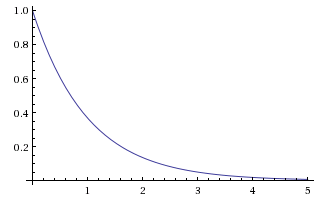
\includegraphics[scale=0.65]{fp-example.png}
    \caption { Exemplo de função de pertinência($\mu_A(x)$) de um elemento x a um conjunto hipotético A, quando esse elemento abrange valores de zero a cinco. }
\end{figure}

Essa teoria se mostra particularmente eficiente ao tratarmos casos onde a transição dos valores de pertinência a certos conjuntos devem ser contínuos, como uma pessoa com febre\cite{Meneghetti:2015}. Seja $F$ o conjunto das pessoas que estão com febre, comumente dizemos que até 37,8ºC, o indivíduo $x$ não participa desse conjunto($\mu_F(x) = 0$) e a partir desse valor, participa desse contjunto($\mu_F(x) = 1$). Obviamente essa descrição não é boa, pois trata por igual aqueles que tem graus de febre diferentes. Neste exemplo, temos a seguinte situação, descrita pelas equações (1) e (2), como também pela figura 2:

\begin{equation}
\mu_F(x) = 0; \forall x < 37.8 ºC
\end{equation}

\begin{equation}
\mu_F(x) = 1; \forall x \geq 37.8 ºC
\end{equation}

\begin{figure}[!ht]
    %figura 2
    \centering
    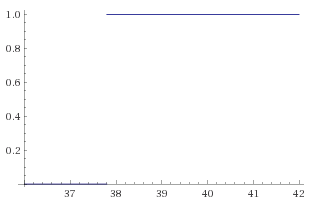
\includegraphics[scale=0.7]{fp-classical.png}
    \caption { Exemplo de função de pertinência clássica($\mu_F(x)$,x) de um elemento temperatura ao conjunto F. }
\end{figure}

%------------------------------------------------

\subsection{Controladores \textit{Fuzzy}}

Os controladores fuzzy são classificados em função do seu método de tomada de decisão e podem ser reunidos em dois grandes grupos. O primeiro modelo (Mamdani) define funções de pertinência para os conjuntos saída e  aplicam um dos métodos de defuzificação tratados adiante para  obter o sinal de controle $u(k)$. Já os do segundo modelo (Sugeno) dispensa a definição de funções de pertinência para os conjuntos de saída e a utilizam como função das entradas. Tendo como entradas do controlador os sinais $a$ e $b$, podemos dizer que o sinal de controle: $u(k)$ $=$ $f(a,b)$.

As funções de pertinência podem ser de vários tipos: degrau, exponencial, gaussiana, triangular, trapezoidal, \textit{Singleton} e \textit{Shouldered}. Na seção de resultados, apresentaremos parâmetros de 3 componentes(quando a função for triangular) e de 4 componentes(quando a função for trapezoidal).

Nos dois tipos de controladores a ação de controle é obtida por meio da definição de um conjunto de instruções (ou regras) de controle. A tabela \ref{table:fuzzyrules} mostra um exemplo de regras de controle.

\begin{table}[!ht]
\caption{Exemplo de regras para um controlador fuzzy de duas entradas,  com três funções de pertinência para cada uma delas - note que as regras podem se repetir em diferentes combinações de entradas, quando necessário}
\label{table:fuzzyrules}
\centering
\begin{tabular}{lllr}
\toprule
\multicolumn{3}{r}{\textbf{$e(k)$}} \\
\cmidrule(r){2-4}
\textbf{$\Delta$e(k)} & \textbf{Negativo} & \textbf{Nulo} & \textbf{Positivo} \\
Negativo & $R_1$ & $R_2$ & $R_3$ \\
Nulo & $R_4$ & $R_5$ & $R_6$ \\
Positivo & $R_7$ & $R_8$ & $R_9$ \\
\bottomrule
\end{tabular}
\end{table}

%------------------------------------------------

\subsection{Controlador Mamdani}

A ação deste controlador é definida pela agregação das n regras $R_i$ que foram ativadas pelas entradas do algoritmo. Esta agregação resulta numa função de inferência do conjunto fuzzy de saída C($\mu_C(x)$). A saída efetiva do controlador(valor numérico) é então obtida por meio de um processo de defuzificação aplicado ao conjunto C. 

As diferentes possibilidades para a implementação dos conectores das regras, das funções de implicação e do processo de defuzificação são amplamente discutidas na literatura (ver, por exemplo, \cite{Lee:1990}.

\subsection{Métodos de defuzificação}

\subsubsection{Centro de área (CoA)}

O método do centro de área é calculado tomando o centro geométrico da função de inferência do conjunto de saída C($\mu_C(x)$) do controlador nebuloso. Apesar de oferecer os melhores resultados, ele não é muito utilizado pois requer alto esforço computacional.

\subsubsection{Média dos máximos (MoM)}

Tomando os valores de máximo da função $\mu_C(x)$ e tirando a média, podemos obter uma boa aproximação para o valor numérico oferecido pelo método do centro de área sem a necessidade de um esforço computacional tão elevado.

\subsection{Controlador Sugeno}

O controlador de Sugeno (ver \cite{TakagiSugeno:1983}) consiste numa simplificação do controlador de Mamdani, onde o conseqüente de cada regra é definido como uma função das variáveis lingüísticas de entrada. Isto é, sejam x(k) e y(k) as entradas do controlador nebuloso e z sua saída, a regra geral $R_i$ pode ser escrita como:\\
Regra($R_i$): se $x$ é $A_i$ e y é $B_i$ então $z$ $=$ $f_i(x,y)$\\
A equação \ref{eq:z} exemplifica uma função de Sugeno bilinear (sistema com duas entradas), com coeficientes $a$, $b$ e $c$.

\begin{equation}
z(k) = f(x(k),y(k)) = ax(k) + by(k) + c
\label{eq:z}
\end{equation}

O resultado de cada regra é, portanto, um valor numérico (não um conjunto fuzzy), que assume como peso o valor da pertinência resultante do processamento do antecedente da regra. Essa determinação dispensa, portanto, a definição de uma função de implicação específica. A resposta final do controlador é obtida pela média ponderada das respostas das regras individuais. Isto é, neste tipo de controlador não cabe processo de defuzificação.

\subsection{Implementação computacional}

Atualmente, alguns programas de uso geral dispõem de módulos específicos para facilitar a implementação computacional das simulações, como é o caso do \textit{Fuzzy Logic Toolbox} do MATLAB\textsuperscript{\textregistered}, usado neste trabalho para implementar os dois tipos de controladores em estudo. O programa permite ao usuário definir os quatro componentes principais do sistema de inferência \textit{fuzzy}, que são: fuzificação dos valores das variáveis de entrada e aplicação dos operadores que podem estar presentes no antecedente das regras (“e” e “ou”); implicação do antecedente sobre o conseqüente (função de implicação); agregação dos conseqüentes de todas as regras definidas; e a defuzificação do conjunto de resposta. No MATLAB\textsuperscript{\textregistered}, antes de iniciar a definição dos componentes do sistema, o usuário deve indicar o tipo do seu controlador, Mamadani ou Sugeno. Dependendo do tipo selecionado, são habilitador os campos pertinentes para a entrada dos dados. Isto é, se for selecionado o controlador de Sugeno, por exemplo, os campos referentes à função de implicação, o termo de agregação “também” e o método de defuzificação ficam desabilitados. O programa apresenta diferentes opções ao usuário para a configuração dos componentes do sistema e, para a maioria dos campos, também permite a definição de outras alternativas.

\section{O problema}\label{problema}

O sistema a ser controlado é o sistema de tanques acoplados da Quanser\textsuperscript{\textregistered}, que tem model matemático dado por:
\begin{equation}
\label{eq:dL1}
\dot{L_{1}} = - \frac{a_{1}}{A_{1}} \sqrt{\frac{g}{2L_{1o}}}L_{1}+\frac{K_{m1}}{A_{1}}V_{p1}
\end{equation}

\begin{equation}
\label{eq:dL2}
\dot{L_{2}} = - \frac{a_{2}}{A_{2}} \sqrt{\frac{g}{2L_{2o}}}L_{2}+\frac{a_{1}}{A_{1}} \sqrt{\frac{g}{2L_{1o}}}L_{1}
\end{equation}

Onde $L_{1}$ e $\dot{L_{1}}$ são o nível do tanque superior e sua variação. O mesmo vale para $L_{2}$ e $\dot{L_{2}}$, para o tanque inferior. As constantes $a_{1}$ e $A_{1}$, assim como $a_{2}$ e $A_{2}$, são as áreas dos orifícios e da seção transversal dos tanques superior e inferior, respectivamente. $V_{p1}$ é a tensão aplicada à bomba e $K_{m1}$ é a constante da bomba. Discretizando o modelo para o período de amostragem da planta (\textit{100 ms}) e aplicando as constantes fornecidas pelo fabricante do experimento temos:

\begin{equation}
\label{eq:discrete}
\begin{cases}
L_{1}(k) = 0,9935 L_{1}(k-1) + 0,0296V_{p1}(k-1) \\
L_{2}(k) = 0,0065L_{1}(k-1)+0,9935L_{2}(k-1)+ \\ 
\hspace{1.33cm}0,0001V_{p1}(k-1)
\end{cases}
\end{equation}


\section{Metodologia}\label{metodologia}

A partir da simulação representada na figura \ref{img:simulink}, realizamos a sintonia de controladores fuzzy do tipo Mamdani e Sugeno.

\begin{figure}[!ht]
    %figura 2
    \centering
    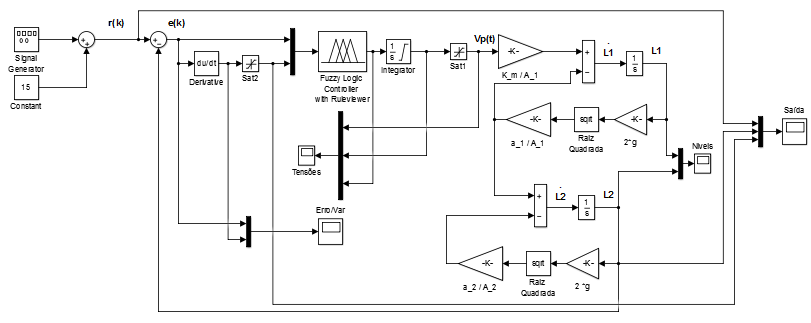
\includegraphics[scale=0.4]{simulink.png}
    \caption { Simulação do sistema de controle \textit{fuzzy} utilizado. }
	\label{img:simulink}
\end{figure}

No controlador desenvolvido foi adotado um método para o processo de decisão baseado em regras do tipo “SE A ENTÃO B”, nas quais tanto o antecedente quanto o conseqüente são valores de variáveis lingüísticas, expressos em conjuntos \textit{fuzzy} como descrito em\cite{MamdaniAssilian:1975}.

De forma suscinta, as funções de pertinência foram incialmente escolhidas empiricamente e refinadas conforme foram sendo realizadas as simulações e observado o comportamento do sistema. Baseado nas funções de pertinência definidas, foi construído o conjunto de regras de inferência, considerando a quantidade de entradas e funções. Em sequência, definiram-se as funções lineares de pertinência da saída, a saber:

\itemize{
\item{MANTER: ação fraca para manutenção do nível do tanque quando nível está próximo ao \textit{setpoint}.}
\item{SUBIR: ação moderada para aumento do nível do tanque quando o nível do tanque está abaixo do \textit{setpoint}, mas convergindo para ele.}
\item{DESCER: ação moderada para redução do nível do tanque quando o nível do tanque está acima do \textit{setpoint}, mas convergindo para ele.}
\item{SUBIR FORTE: ação intensa para aumento do nível do tanque quando o nível está divergindo decrescentemente do \textit{setpoint}.}
\item{DESCER FORTE: ação intensa para redução do nível do tanque quando o nível está divergindo crescentemente do \textit{setpoint}.}
}

O parâmetros de controle definidos para cada umas das funções de saída, expresso por um vetor de saída com 3 elementos, onde o primeiro comporta-se como o fator integrativo, o segundo como o proporcional e o terceiro como uma constante de \textit{offset} do modelo clássico da teoria de controle. Os valores foram escolhidos pela observação do comportamento da simulação.

%As tabelas \ref{tab:rulesMamdani0}, \ref{tab:pertinenceMamdani0}, e \ref{tab:inferenceMamdani0}, representam respectivamente, as regras para o controlador Mamdani, os parâmetros de pertinência para a entrada $e(k)$ e $\Delta$e(k) e os parâmetros de inferência de saída $u(k)$, enquanto a figura 4 mostra o comportamento do nível do tanque 2(variável manipulada) em relação ao nosso referencial

\subsection{Modelo Sugeno}

Mesmo com a saturação do sinal da bomba, limitado a $\pm4$, o overshoot somente foi sanado com a ação da integração do erro quando o sinal da bomba entrava em saturação. Esta técnica é documentada na literatura como \textit{anti-windup}\footnote{\url{https://en.wikipedia.org/wiki/Integral_windup}}.

A determinação dos parâmetros proporcional, integrativo e da constante foi feita de forma empírica.

\subsection{Modelo Mamdani}

A escolhas das regras seguiu os mesmos procedimentos do Sugeno, com exceção da saída que tem três funções de pertinência triangulares (MANTER, SUBIR E DESCER), nos quais definiram-se os valores de incremento do sinal de controle.

Foram realizados dois testes. Um com as funções de saída simétricas e funções de pertinência do erro deslocadas para a esquerda para compensar a vazão dos orifícios de saída dos tanques (teste 1). O segundo teste foi feito o inverso, as funcções de pertinência do erro foram simétricas e as funões de saída foram deslocadas à direita para, novamente, estabilizar o nível do tanque compensando a vazão de saída (teste 2). O terceiro teste foi feito deslocando as funções de pertinência do erro para a esquerda e as funões de saída foram deslocadas à direita para, novamente, estabilizar o nível do tanque compensando a vazão de saída (teste 3).

\section{Resultados}\label{resultados}

\subsection{Mamdani - melhor resultado}

As tabelas \ref{tab:rulesMamdani0}, \ref{tab:pertinenceMamdani0} e \ref{tab:inferenceMamdani0} apresentam respectivamente, as regras para o controlador Mamdani, os parâmetros de pertinência para a entrada $e(k)$ e para $\Delta$e(k) e os parâmetros de inferência de saída $u(k)$, enquanto a figura \ref{fig:resultMamdani0} mostra o comportamento da variável manipulada (nível do tanque 2) em relação ao \textit{setpoint} (referencial).

\begin{table}[!ht]
\caption{Regras dos controladores Mamdani}
\label{tab:rulesMamdani0}
\centering
\begin{tabular}{lllr}
\toprule
\multicolumn{3}{r}{\textbf{$e(k)$}} \\
\cmidrule(r){2-4}
\textbf{$\Delta$e(k)} & \textbf{Negativo} & \textbf{Nulo} & \textbf{Positivo} \\
Negativo & Descer & Descer & Subir \\
Nulo & Descer & Manter & Subir \\
Positivo & Descer & Subir & Subir \\
\bottomrule
\end{tabular}
\end{table}

%---------------------------------

\begin{table}[!ht]
\caption{Parâmetros de pertinência do erro (Mamdani)}
\label{tab:pertinenceMamdani0}
\centering
\begin{tabular}{lrr}
\toprule
& \multicolumn{1}{c}{$e(k)$} & \multicolumn{1}{c}{$\Delta$e(k)} \\
\cmidrule(r){1-3}
Negativo & [-54 -30 -3] & [-1.8 -1 0] \\
Nulo & [-5 -2.2 0.5] & [-0.2 -0 0.2] \\
Positivo & [-2 30 54] & [0 1 1.8] \\
\bottomrule
\end{tabular}
\end{table}

%---------------------------------

\begin{table}[!ht]
\caption{Parâmetros de inferência de saída (Mamdani)}
\label{tab:inferenceMamdani0}
\centering
\begin{tabular}{lr}
\toprule
\multicolumn{2}{c}{$u(k)$} \\
\cmidrule(r){1-2}
Descer & [-4 -2 -1] \\
Manter & [-1 -0 1] \\
Subir & [1 2 4] \\
\bottomrule
\end{tabular}
\end{table}

%---------------------------------

\begin{figure}[!ht]
    %figura 2
    \centering
    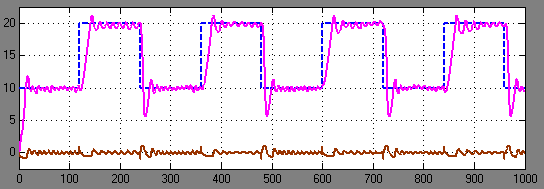
\includegraphics[width=\columnwidth]{mamdani1.png}
    \caption { Melhor resultado (Mamdani) }
	\label{fig:resultMamdani0}
\end{figure}

%---------------------------------

\subsection{Mamdani - outros testes}

Esta seção são apresentados outros testes realizados usando diferentes configurações para o controlador Mamdani. As regras de controle foram mantidas as mesmas, alterando apenas os valores para funções de pertinência e inferência.

\begin{table}[!h]
\caption{Parâmetros de pertinência do 2o. teste \\ (Mamdani)}
\centering
\begin{tabular}{lrr}
\toprule
& \multicolumn{1}{c}{$e(k)$} & \multicolumn{1}{c}{$\Delta$e(k)} \\
\cmidrule(r){1-3} 
Negativo & [-540 -10 -1] & [-10 -1 -0.1] \\
Nulo & [-2 0 2] & [-0.2 -0 0.2] \\
Positivo & [1 10 540] & [0 1 10.8] \\
\bottomrule
\end{tabular}
\end{table}

\begin{table}[!h]
\caption{Parâmetros de inferência de saída do 2o. teste \\ (Mamdani)}
\centering
\begin{tabular}{lr}
\toprule
\multicolumn{2}{c}{$u(k)$} \\
\cmidrule(r){1-2}
Descer & [-8 -2 -1] \\
Manter & [-1 -0 1] \\
Subir & [1 2 4] \\
\bottomrule
\end{tabular}
\end{table}

\begin{figure}[!h]
    %figura 2
    \centering
    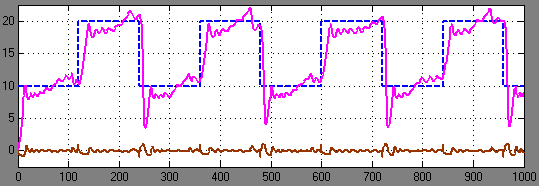
\includegraphics[width=\columnwidth]{mamdani2.png}
    \caption { Resultado para o do 2o. teste (Mamdani)}
\end{figure}

Neste segundo teste do controlador Mamdani, houve um \textit{undershoot} na descida maior que no melhor caso uma antecipação da subida, cuja causa não foi investigada. O acompanhamento do \textit{setpoint}, no entanto, tende a seguir a referência, mas com alguma divergência.

\begin{table}[!h]
\caption{Parâmetros de pertinência do 3o. teste \\ (Mamdani)}
\centering
\begin{tabular}{lrr}
\toprule
& \multicolumn{1}{c}{$e(k)$} & \multicolumn{1}{c}{$\Delta$e(k)} \\
\cmidrule(r){1-3} 
Negativo & [-540 -20 -2] & [-10 -1 0.01] \\
Nulo & [-3.5 -1 1] & [-0.2 -0 0.2] \\
Positivo & [0 10 540] & [0.01 1 10.8] \\
\bottomrule
\end{tabular}
\end{table}

\begin{table}[!h]
\caption{Parâmetros de inferência de saída do 3o. teste (Mamdani)}
\centering
\begin{tabular}{lr}
\toprule
\multicolumn{2}{c}{$u(k)$} \\
\cmidrule(r){1-2}
Descer Forte & [-12 -4 1] \\
Descer & [-2 -1.5 -0.1] \\
Manter & [-0.6 0.1 0.5] \\
Subir & [0.1 1.25 2.25] \\
Subir Forte & [1 4 12] \\
\bottomrule
\end{tabular}
\end{table}

\begin{figure}[!h]
    %figura 2
    \centering
    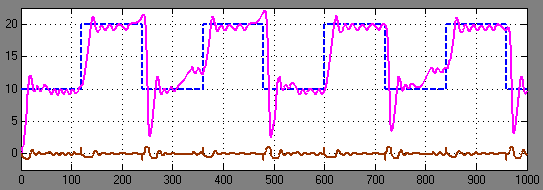
\includegraphics[width=\columnwidth]{mamdani3.png}
    \caption { Resultado para do 3o. teste (Mamdani)}
\end{figure}

Como pode-se observar, no terceiro teste do controlador Mamdani, houve um \textit{undershoot} na descida maior que no teste anterior e, novamente, uma antecipação da subida, cuja causa também não foi investigada. O acompanhamento do \textit{setpoint}, no entanto, tende a seguir mais detidamente a referência.

%---------------------------------

\subsection{Sugeno - melhor resultado}

As tabelas \ref{tab:rulesSugeno0}, \ref{tab:pertinenceSugeno0} e \ref{tab:bilinearSugeno0} representam respectivamente, as regras para o controlador Sugeno, os parâmetros de pertinência para a entrada $e(k)$ e para $\Delta$e(k) e os parâmetros de inferência de saída $u(k)$, enquanto a figura \ref{fig:resultSugeno0} mostra o comportamento da variável manipulada (nível do tanque 2) em relação ao \textit{setpoint} (referencial).

%-------------------------------------------------

\begin{table}[!h]
\caption{Regras dos controladores do melhor resultado (Sugeno)}
\label{tab:rulesSugeno0}
\centering
\begin{tabular}{lllr}
\toprule
\multicolumn{3}{r}{\textbf{$e(k)$}} \\
\cmidrule(r){2-4}
\textbf{$\Delta$e(k)} & \textbf{Negativo} & \textbf{Nulo} & \textbf{Positivo} \\
Negativo & $D_f$ & M & S \\
Nulo & D & M & S \\
Positivo & D & M & $S_f$ \\
\bottomrule
\end{tabular}
\end{table}

%-------------------------------------------------

\begin{table}[!h]
\caption{Parâmetros de pertinência do melhor resultado (Sugeno)}
\label{tab:pertinenceSugeno0}
\centering
\begin{tabular}{lrr}
\toprule
& \multicolumn{1}{c}{$e(k)$} & \multicolumn{1}{c}{$\Delta$e(k)} \\
\cmidrule(r){1-3}
Negativo & [-4970 -4970 -8 -1] & [-2 -1 0.104] \\
Nulo & [-3 0 1] & [-0.2 0 0.1] \\
Positivo & [0 6 30 5500] & [0 1 2] \\
\bottomrule
\end{tabular}
\end{table}

%-------------------------------------------------

\begin{table}[!h]
\caption{Parâmetros das funções bilineares de saída do melhor resultado (Sugeno)}
\label{tab:bilinearSugeno0}
\centering
\begin{tabular}{lr}
\toprule
\multicolumn{2}{c}{$u(k)$} \\
\cmidrule(r){1-2}
Descer Forte & [0.1 10 0] \\
Descer & [0.09 1.5 0] \\
Manter & [0.05 1 0] \\
Subir & [0.08 3 0] \\
Subir Forte & [0.05 2.5 0] \\
\bottomrule
\end{tabular}
\end{table}

%-------------------------------------------------

\begin{figure}[!h]
    %figura 2
    \centering
    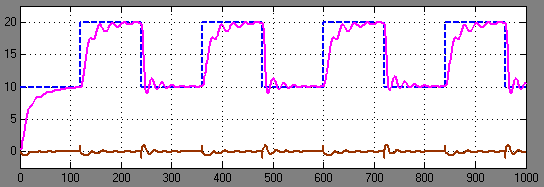
\includegraphics[width=\columnwidth]{sugeno1.png}
    \caption { Melhor resultado (Sugeno)}
    \label{fig:resultSugeno0}
\end{figure}

%------------------------------------------------

\subsection{Outros testes - Sugeno}

Esta seção abordará outros testes, realizados usando diferentes configurações Sugeno. As regras de controle foram mantidas as mesmas, alterando apenas os valores para funções de pertinência e parâmetros das funções bilineares.

\begin{table}[!h]
\caption{Parâmetros de pertinência do 2o. teste \\ (Sugeno)}
\centering
\begin{tabular}{lrr}
\toprule
& \multicolumn{1}{c}{$e(k)$} & \multicolumn{1}{c}{$\Delta$e(k)} \\
\cmidrule(r){1-3} 
Negativo & [-4970 -4970 -10 -1] & [-2 -1 0.104] \\
Nulo & [-5 0 5] & [-0.2 0 0.2] \\
Positivo & [1 10 30 5500] & [0 1 2] \\
\bottomrule
\end{tabular}
\end{table}

\begin{table}[!h]
\caption{Parâmetros das funções bilineares de saída do 2o. teste (Sugeno)}
\centering
\begin{tabular}{lr}
\toprule
\multicolumn{2}{c}{$u(k)$} \\
\cmidrule(r){1-2}
Descer Forte & [0.5 10 0] \\
Descer & [0.18 3 0] \\
Manter & [0.04 0.55 0] \\
Subir & [0.08 2 0] \\
Subir Forte & [0.05 2.5 0] \\
\bottomrule
\end{tabular}
\end{table}

\begin{figure}[!h]
    %figura 2
    \centering
    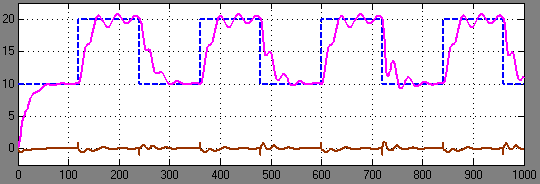
\includegraphics[width=\columnwidth]{sugeno2.png}
    \caption { Resultado do 2o. teste (Sugeno) }
\end{figure}

Como pode-se observar, no segundo teste, houve um retardo no acompanhamento do \textit{setpoint} tanto na subida quanto na descida da referência.

\begin{table}[!h]
\caption{Parâmetros de pertinência do 3o. teste \\ (Sugeno)}
\centering
\begin{tabular}{lrr}
\toprule
& \multicolumn{1}{c}{$e(k)$} & \multicolumn{1}{c}{$\Delta$e(k)} \\
\cmidrule(r){1-3} 
Negativo & [-543 -87 -15 -3.5] & [-10 -1 -0.08] \\
Nulo & [-5 1.15 3] & [-0.15 0 0.08] \\
Positivo & [2 15 87 543] & [0.06 1 5] \\
\bottomrule
\end{tabular}
\end{table}

\begin{table}[!h]
\caption{Parâmetros das funções bilineares de saída do 3o. teste (Sugeno)}
\centering
\begin{tabular}{lr}
\toprule
\multicolumn{2}{c}{$u(k)$} \\
\cmidrule(r){1-2}
Descer Forte & [0.5 10 0] \\
Descer & [0.3 10 0] \\
Manter & [0.045 1.7 0] \\
Subir & [0.19 6.5 0] \\
Subir Forte & [0.25 3.8 0] \\
\bottomrule
\end{tabular}
\end{table}

\begin{figure}[!h]
    %figura 2
    \centering
    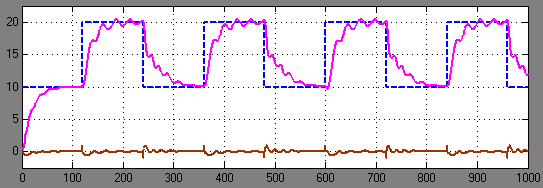
\includegraphics[width=\columnwidth]{sugeno3.png}
    \caption { Resultado para o do 3o. teste (Sugeno)}
\end{figure}

Neste terceiro teste, percebemos um aumento da lentidão do sistema em acompanhar o \textit{setpoint} tanto na subida quanto na descida da referência.

%------------------------------------------------

\section{Conclusões}\label{conclusoes}

Analisando as figuras \ref{fig:resultMamdani0} e \ref{fig:resultSugeno0}, podemos observar que,  apesar de mais complexo, o controlador Mamdani reagiu melhor ao sistema, com um tempo de acomodação consideravelmente menor. Entretanto, este apresenta um valor de \textit{overshoot}, que é menor nos controladores Sugeno. Observa-se, também, que o controlador Mamdani apresenta uma oscilação em torno do \textit{setpoint}, oscilação de ciclo limite. Esta oscilação poderia ser eliminada utilizando um controlador Sugeno, considerando o melhor controle sobre as ações integrativas.

A quantidade de funções de pertinência, no caso deste estudo -- cinco, gera conjuntos \textit{fuzzy} menos refinados e, portanto, aciona as regras de controle com variações maiores de valores que pode acarretar em ações de controle excessivamente agressivas. Outro parâmetro a se observar é amplitude de variação do sinal de controle, que a depender do passo de integração pode levar ao crescimento excessivo do sinal de controle por efeito integrativo. Neste trabalho, a solução para obtermos tempo de estabilização menores usando amplitudes de incrememento maiores foi o uso de um supressor de integração documentado na literatura como \textit{anti-windup}.

Pôde-se perceber que o número de funções de pertinência deve ser avaliado com cautela durante o projeto do controlador. O problema de controle proposto mostrou-se mais difícil de parametrizar com uma quantidade reduzida de funções de pertinência e ações de controle, no caso do Mamdani, dadas as variações no incremento da ação de controle, que em algum momento pode ser de grande amplitude se apenas algumas ações forem definidas.

A exploração dos parâmetros de controle permitiu uma aquisição de experiência inicial na configuração de controladores \textit{fuzzy}, mesmo que inicial, aos integrantes da equipe, mas relevante na composição de conhecimentos no domínio de sistemas de controle.

%----------------------------------------------------------------------------------------
%	REFERENCIAS
%----------------------------------------------------------------------------------------

\begin{thebibliography}{99} % Bibliography 

\bibitem[Lee, 1990]{Lee:1990}
Lee, C. C. (1990).
\newblock Fuzzy Logic in Control Systems: Fuzzy Logic Controller.
\newblock {\em Part I. IEEE Transactions on Systems, Man, and Cybernetics}, Vol. 20, No. 2, March/April 1990, pp. 404 – 418.

\bibitem[Mamdani, 1973]{Mamdani:1973}
Mamdani, E. H. e Assilian S. (1973)
\newblock Aplications of fuzzy algorithms for control of simple dynamic plant.
\newblock {\em Proc. IEEE 121}, vol. 12, p. 1585-1588.

\bibitem[Mamdani e Assilian, 1975]{MamdaniAssilian:1975}
Mamdani, E. H. e Assilian S. (1975).
\newblock An experiment in linguistic synthesis with a fuzzy logic controller.
\newblock {\em International Journal Man-Machine Studies}, vol. 7, p. 1-13.

\bibitem[Meneghetti, 2015]{Meneghetti:2015}
Meneghetti, F. M. U. A. (2015).
\newblock Controle Inteligente.
\newblock {\em Material de apoio da disciplina de Controle Inteligente}.

\bibitem[Sugeno, 1985]{Sugeno:1985}
Sugeno, M. (1985).
\newblock An introductory survey of fuzzy control.
\newblock {\em Information Sciences}, No. 36, p. 59-83.

\bibitem[Takagi e Sugeno, 1983]{TakagiSugeno:1983}
Takagi, T. e Sugeno M. (1983).
\newblock Derivation of fuzzy control rules from human operator’s control action.
\newblock {\em IFAC Symposium on Fuzzy Information, Knowledge Representation and Decision Analysis}, Marseille, p. 55-60.

\bibitem[Zadeh, 1965]{Zadeh:1965}
Zadeh, L. A. (1965).
\newblock Fuzzy Sets.
\newblock {\em INFORMATION AND CONTROL}, No. 8, p. 338-353.

\bibitem[Zadeh, 1973]{Zadeh:1973}
Zadeh, L. A. (1973).
\newblock Outline of a new approach to the analysis of complex systems and decision processes.
\newblock {\em IEEE Transactions on Systems, Man, and Cybernetics}, Vol. SMC-3, No. 1, p. 28-44.

\bibitem[Zimmermann, 1996]{Zimmermann:1996}
Zimmermann, H.-J. (1996).
\newblock Fuzzy Set Theory and Its Applications.
\newblock {\em 3rd Edition. Kluwer Academic Publishers}.

\end{thebibliography}

%----------------------------------------------------------------------------------------

\end{document}
